\documentclass{article}\usepackage[]{graphicx}\usepackage[]{color}
%% maxwidth is the original width if it is less than linewidth
%% otherwise use linewidth (to make sure the graphics do not exceed the margin)
\makeatletter
\def\maxwidth{ %
  \ifdim\Gin@nat@width>\linewidth
    \linewidth
  \else
    \Gin@nat@width
  \fi
}
\makeatother

\definecolor{fgcolor}{rgb}{0.345, 0.345, 0.345}
\newcommand{\hlnum}[1]{\textcolor[rgb]{0.686,0.059,0.569}{#1}}%
\newcommand{\hlstr}[1]{\textcolor[rgb]{0.192,0.494,0.8}{#1}}%
\newcommand{\hlcom}[1]{\textcolor[rgb]{0.678,0.584,0.686}{\textit{#1}}}%
\newcommand{\hlopt}[1]{\textcolor[rgb]{0,0,0}{#1}}%
\newcommand{\hlstd}[1]{\textcolor[rgb]{0.345,0.345,0.345}{#1}}%
\newcommand{\hlkwa}[1]{\textcolor[rgb]{0.161,0.373,0.58}{\textbf{#1}}}%
\newcommand{\hlkwb}[1]{\textcolor[rgb]{0.69,0.353,0.396}{#1}}%
\newcommand{\hlkwc}[1]{\textcolor[rgb]{0.333,0.667,0.333}{#1}}%
\newcommand{\hlkwd}[1]{\textcolor[rgb]{0.737,0.353,0.396}{\textbf{#1}}}%

\usepackage{framed}
\makeatletter
\newenvironment{kframe}{%
 \def\at@end@of@kframe{}%
 \ifinner\ifhmode%
  \def\at@end@of@kframe{\end{minipage}}%
  \begin{minipage}{\columnwidth}%
 \fi\fi%
 \def\FrameCommand##1{\hskip\@totalleftmargin \hskip-\fboxsep
 \colorbox{shadecolor}{##1}\hskip-\fboxsep
     % There is no \\@totalrightmargin, so:
     \hskip-\linewidth \hskip-\@totalleftmargin \hskip\columnwidth}%
 \MakeFramed {\advance\hsize-\width
   \@totalleftmargin\z@ \linewidth\hsize
   \@setminipage}}%
 {\par\unskip\endMakeFramed%
 \at@end@of@kframe}
\makeatother

\definecolor{shadecolor}{rgb}{.97, .97, .97}
\definecolor{messagecolor}{rgb}{0, 0, 0}
\definecolor{warningcolor}{rgb}{1, 0, 1}
\definecolor{errorcolor}{rgb}{1, 0, 0}
\newenvironment{knitrout}{}{} % an empty environment to be redefined in TeX

\usepackage{alltt}
\usepackage{geometry}
\usepackage{amsmath}
\usepackage{lscape}
\geometry{verbose,tmargin=2.5cm,bmargin=2.5cm,lmargin=2.5cm,rmargin=2.5cm}
\IfFileExists{upquote.sty}{\usepackage{upquote}}{}
\begin{document}




\title{Messina E2B: MessinaSurv vs Others}
\maketitle


%%%%%%%%%%%%%%%%%%%%%%%%%%%%%%%%%%%%%%%%%%%%%%%%%%%%%%%%%%%%%%%%%%%%%%
% LIBRARIES
%%%%%%%%%%%%%%%%%%%%%%%%%%%%%%%%%%%%%%%%%%%%%%%%%%%%%%%%%%%%%%%%%%%%%%
\section{Preparation}
\begin{knitrout}
\definecolor{shadecolor}{rgb}{0.969, 0.969, 0.969}\color{fgcolor}\begin{kframe}
\begin{alltt}
\hlkwd{library}\hlstd{(plyr)}
\hlkwd{library}\hlstd{(messina)}
\hlkwd{library}\hlstd{(maxstat)}
\hlkwd{library}\hlstd{(doMC)}

\hlstd{deltaForMargin} \hlkwb{=} \hlkwa{function}\hlstd{(}\hlkwc{margin}\hlstd{,} \hlkwc{sigma_epsilon} \hlstd{=} \hlnum{1}\hlstd{,} \hlkwc{alpha} \hlstd{=} \hlnum{0.05}\hlstd{) margin} \hlopt{-} \hlnum{2}\hlopt{*}\hlstd{sigma_epsilon}\hlopt{*}\hlkwd{qnorm}\hlstd{(alpha)}
\hlstd{marginForDelta} \hlkwb{=} \hlkwa{function}\hlstd{(}\hlkwc{delta}\hlstd{,} \hlkwc{sigma_epsilon} \hlstd{=} \hlnum{1}\hlstd{,} \hlkwc{alpha} \hlstd{=} \hlnum{0.05}\hlstd{) delta} \hlopt{+} \hlnum{2}\hlopt{*}\hlstd{sigma_epsilon}\hlopt{*}\hlkwd{qnorm}\hlstd{(alpha)}

\hlstd{messina_objectives} \hlkwb{=} \hlkwd{list}\hlstd{(}\hlstr{"cox.log2"} \hlstd{=} \hlkwd{messinaSurvObj.CoxCoef}\hlstd{(}\hlkwd{log}\hlstd{(}\hlnum{2}\hlstd{)))}

\hlstd{e2b.design} \hlkwb{=} \hlkwd{expand.grid}\hlstd{(}
        \hlkwc{Delta} \hlstd{=} \hlkwd{seq}\hlstd{(}\hlnum{0}\hlstd{,} \hlnum{5}\hlstd{,} \hlnum{0.5}\hlstd{),}
        \hlkwc{R1} \hlstd{=} \hlkwd{c}\hlstd{(}\hlnum{1}\hlstd{,} \hlnum{2}\hlstd{,} \hlnum{4}\hlstd{,} \hlnum{8}\hlstd{,} \hlnum{16}\hlstd{),}
        \hlkwc{sigma_epsilon} \hlstd{=} \hlnum{1}\hlstd{,}
        \hlkwc{p1} \hlstd{=} \hlkwd{c}\hlstd{(}\hlnum{0.2}\hlstd{,} \hlnum{0.5}\hlstd{,} \hlnum{0.8}\hlstd{),}
        \hlkwc{pc} \hlstd{=} \hlkwd{c}\hlstd{(}\hlnum{0}\hlstd{,} \hlnum{0.2}\hlstd{,} \hlnum{0.5}\hlstd{),}
        \hlkwc{alpha} \hlstd{=} \hlnum{0.2}\hlstd{,}
        \hlkwc{stat.alpha} \hlstd{=} \hlnum{0.05}\hlstd{,}
        \hlkwc{messina.objective} \hlstd{=} \hlstr{"cox.log2"}\hlstd{,}
        \hlkwc{messina.minmarg} \hlstd{=} \hlnum{1}\hlstd{,}
        \hlkwc{n} \hlstd{=} \hlkwd{c}\hlstd{(}\hlnum{25}\hlstd{,} \hlnum{50}\hlstd{,} \hlnum{100}\hlstd{),}
        \hlkwc{reps} \hlstd{=} \hlnum{5e1}\hlstd{)}

\hlstd{e2b.design}\hlopt{$}\hlstd{margin} \hlkwb{=} \hlkwd{marginForDelta}\hlstd{(e2b.design}\hlopt{$}\hlstd{Delta, e2b.design}\hlopt{$}\hlstd{sigma_epsilon,} \hlkwc{alpha} \hlstd{= e2b.design}\hlopt{$}\hlstd{alpha)}

\hlstd{detector_multicut} \hlkwb{=} \hlkwa{function}\hlstd{(}\hlkwc{x}\hlstd{,} \hlkwc{y}\hlstd{,} \hlkwc{ncuts} \hlstd{=} \hlnum{10}\hlstd{,} \hlkwc{correct} \hlstd{=} \hlstr{"none"}\hlstd{)}
\hlstd{\{}
        \hlkwa{if} \hlstd{(ncuts} \hlopt{==} \hlnum{1}\hlstd{)         \{ correct} \hlkwb{=} \hlstr{"none"} \hlstd{\}}
        \hlkwa{if} \hlstd{(}\hlkwd{is.vector}\hlstd{(x))       \{ x} \hlkwb{=} \hlkwd{matrix}\hlstd{(x,} \hlkwc{nrow} \hlstd{=} \hlnum{1}\hlstd{) \}}

        \hlkwd{aaply}\hlstd{(x,} \hlnum{1}\hlstd{,} \hlkwa{function}\hlstd{(}\hlkwc{x1}\hlstd{) \{}
                \hlstd{cutpoints} \hlkwb{=} \hlkwd{quantile}\hlstd{(x1,} \hlkwc{probs} \hlstd{= (}\hlnum{1}\hlopt{:}\hlstd{ncuts)}\hlopt{/}\hlstd{(ncuts} \hlopt{+} \hlnum{1}\hlstd{))}
                \hlstd{pvals} \hlkwb{=} \hlkwd{sapply}\hlstd{(cutpoints,} \hlkwa{function}\hlstd{(}\hlkwc{c}\hlstd{) \{}
                        \hlstd{x1c} \hlkwb{=} \hlstd{x1} \hlopt{>} \hlstd{c}
                        \hlstd{test} \hlkwb{=} \hlkwd{survdiff}\hlstd{(y} \hlopt{~} \hlstd{x1c)}
                        \hlstd{pval} \hlkwb{=} \hlkwd{pchisq}\hlstd{(test}\hlopt{$}\hlstd{chisq,} \hlkwc{df} \hlstd{=} \hlnum{1}\hlstd{,} \hlkwc{lower.tail} \hlstd{=} \hlnum{FALSE}\hlstd{)}
                        \hlstd{pval}
                \hlstd{\})}
                \hlstd{pvals} \hlkwb{=} \hlkwd{p.adjust}\hlstd{(pvals, correct)}
                \hlstd{pvals[}\hlkwd{is.na}\hlstd{(pvals)]} \hlkwb{=} \hlnum{1}
                \hlkwd{min}\hlstd{(pvals)}
        \hlstd{\},} \hlkwc{.parallel} \hlstd{=} \hlnum{FALSE}\hlstd{)}
\hlstd{\}}

\hlstd{e2b.datafun} \hlkwb{=} \hlkwa{function}\hlstd{(}\hlkwc{n}\hlstd{,} \hlkwc{p1}\hlstd{,} \hlkwc{pc}\hlstd{,} \hlkwc{Delta}\hlstd{,} \hlkwc{R1}\hlstd{,} \hlkwc{sigma_epsilon}\hlstd{,} \hlkwc{...}\hlstd{)}
\hlstd{\{}
        \hlstd{n1} \hlkwb{=} \hlkwd{round}\hlstd{(n}\hlopt{*}\hlstd{p1)}
        \hlstd{n0} \hlkwb{=} \hlstd{n} \hlopt{-} \hlstd{n1}
        \hlstd{c} \hlkwb{=} \hlkwd{rep}\hlstd{(}\hlkwd{c}\hlstd{(}\hlnum{0}\hlstd{,} \hlnum{1}\hlstd{),} \hlkwd{c}\hlstd{(n0, n1))}
        \hlstd{x} \hlkwb{=} \hlstd{Delta}\hlopt{*}\hlstd{c} \hlopt{+} \hlkwd{rnorm}\hlstd{(n,} \hlkwc{mean} \hlstd{=} \hlnum{0}\hlstd{,} \hlkwc{sd} \hlstd{= sigma_epsilon)}

        \hlstd{Rc} \hlkwb{=} \hlkwd{optimize}\hlstd{(}\hlkwa{function}\hlstd{(}\hlkwc{Rc}\hlstd{)} \hlkwd{abs}\hlstd{(}\hlkwd{integrate}\hlstd{(}\hlkwa{function}\hlstd{(}\hlkwc{t}\hlstd{)} \hlkwd{pexp}\hlstd{(t, Rc)} \hlopt{*} \hlstd{((}\hlnum{1}\hlopt{-}\hlstd{p1)}\hlopt{*}\hlkwd{dexp}\hlstd{(t,} \hlnum{1}\hlstd{)} \hlopt{+} \hlstd{p1}\hlopt{*}\hlkwd{dexp}\hlstd{(t, R1)),} \hlnum{0}\hlstd{,} \hlnum{Inf}\hlstd{)}\hlopt{$}\hlstd{value} \hlopt{-} \hlstd{pc),} \hlkwc{interval} \hlstd{=} \hlkwd{c}\hlstd{(R1}\hlopt{/}\hlnum{100}\hlstd{, R1}\hlopt{*}\hlnum{100}\hlstd{))}\hlopt{$}\hlstd{minimum}

        \hlstd{time_event} \hlkwb{=} \hlkwd{c}\hlstd{(}\hlkwd{rexp}\hlstd{(n0,} \hlnum{1}\hlstd{),} \hlkwd{rexp}\hlstd{(n1, R1))}
        \hlstd{time_cens} \hlkwb{=} \hlkwd{rexp}\hlstd{(n, Rc)}

        \hlstd{y} \hlkwb{=} \hlkwd{Surv}\hlstd{(}\hlkwd{pmin}\hlstd{(time_event, time_cens), time_event} \hlopt{<=} \hlstd{time_cens)}

        \hlkwd{list}\hlstd{(}\hlkwc{x} \hlstd{= x,} \hlkwc{y} \hlstd{= y,} \hlkwc{c} \hlstd{= c)}
\hlstd{\}}

\hlstd{e2b.detfun} \hlkwb{=} \hlkwa{function}\hlstd{(}\hlkwc{x}\hlstd{,} \hlkwc{y}\hlstd{,} \hlkwc{stat.alpha}\hlstd{,} \hlkwc{messina.objective}\hlstd{,} \hlkwc{messina.minmarg}\hlstd{,} \hlkwc{...}\hlstd{)}
\hlstd{\{}
        \hlstd{data.maxstat} \hlkwb{=} \hlkwd{data.frame}\hlstd{(}\hlkwc{time} \hlstd{= y[,}\hlnum{1}\hlstd{],} \hlkwc{event} \hlstd{= y[,}\hlnum{2}\hlstd{],} \hlkwc{x} \hlstd{= x)}
        \hlstd{test.maxstat} \hlkwb{=} \hlkwd{try}\hlstd{(}\hlkwd{maxstat.test}\hlstd{(}\hlkwd{Surv}\hlstd{(time, event)} \hlopt{~} \hlstd{x,} \hlkwc{data} \hlstd{= data.maxstat,} \hlkwc{smethod} \hlstd{=} \hlstr{"LogRank"}\hlstd{,} \hlkwc{pmethod} \hlstd{=} \hlstr{"HL"}\hlstd{))}
        \hlstd{det.maxstat} \hlkwb{=} \hlkwd{ifelse}\hlstd{(}\hlkwd{class}\hlstd{(test.maxstat)} \hlopt{==} \hlstr{"try-error"}\hlstd{,} \hlnum{FALSE}\hlstd{, test.maxstat}\hlopt{$}\hlstd{p.value} \hlopt{<} \hlstd{stat.alpha)}

        \hlstd{det.1cut} \hlkwb{=} \hlkwd{detector_multicut}\hlstd{(x, y,} \hlnum{1}\hlstd{)} \hlopt{<} \hlstd{stat.alpha}
        \hlstd{det.10cut} \hlkwb{=} \hlkwd{detector_multicut}\hlstd{(x, y,} \hlnum{10}\hlstd{)} \hlopt{<} \hlstd{stat.alpha}
        \hlstd{det.10cutHolm} \hlkwb{=} \hlkwd{detector_multicut}\hlstd{(x, y,} \hlnum{10}\hlstd{,} \hlstr{"holm"}\hlstd{)} \hlopt{<} \hlstd{stat.alpha}

        \hlstd{x.messina} \hlkwb{=} \hlkwd{rbind}\hlstd{(x, x, x)}
        \hlstd{fit.messina} \hlkwb{=} \hlkwd{messinaSurv}\hlstd{(x.messina, y, messina_objectives[[messina.objective]],} \hlkwc{silent} \hlstd{=} \hlnum{TRUE}\hlstd{,} \hlkwc{parallel} \hlstd{=} \hlnum{FALSE}\hlstd{)}
        \hlstd{det.messina} \hlkwb{=} \hlstd{fit.messina}\hlopt{@}\hlkwc{fits}\hlopt{@}\hlkwc{summary}\hlopt{$}\hlstd{passed[}\hlnum{1}\hlstd{]} \hlopt{==} \hlnum{TRUE} \hlopt{&&} \hlstd{fit.messina}\hlopt{@}\hlkwc{fits}\hlopt{@}\hlkwc{summary}\hlopt{$}\hlstd{margin[}\hlnum{1}\hlstd{]} \hlopt{>=} \hlstd{messina.minmarg}
        \hlstd{det.messina.nomarg} \hlkwb{=} \hlstd{fit.messina}\hlopt{@}\hlkwc{fits}\hlopt{@}\hlkwc{summary}\hlopt{$}\hlstd{passed[}\hlnum{1}\hlstd{]} \hlopt{==} \hlnum{TRUE}

        \hlkwd{c}\hlstd{(}\hlkwc{maxstat} \hlstd{= det.maxstat,} \hlkwc{c1} \hlstd{= det.1cut,} \hlkwc{c10} \hlstd{= det.10cut,} \hlkwc{cH10} \hlstd{= det.10cutHolm,} \hlkwc{m} \hlstd{= det.messina,} \hlkwc{mnm} \hlstd{= det.messina.nomarg)}
\hlstd{\}}

\hlstd{e2b.repfun} \hlkwb{=} \hlkwa{function}\hlstd{(}\hlkwc{i}\hlstd{,} \hlkwc{Delta}\hlstd{,} \hlkwc{R1}\hlstd{,} \hlkwc{sigma_epsilon}\hlstd{,} \hlkwc{pc}\hlstd{,} \hlkwc{p1}\hlstd{,} \hlkwc{stat.alpha}\hlstd{,} \hlkwc{messina.minmarg}\hlstd{,} \hlkwc{messina.objective}\hlstd{,} \hlkwc{n}\hlstd{,} \hlkwc{...}\hlstd{)}
\hlstd{\{}
        \hlstd{data} \hlkwb{=} \hlkwd{e2b.datafun}\hlstd{(n, p1, pc, Delta, R1, sigma_epsilon)}
        \hlstd{dets} \hlkwb{=} \hlkwd{try}\hlstd{(}\hlkwd{e2b.detfun}\hlstd{(data}\hlopt{$}\hlstd{x, data}\hlopt{$}\hlstd{y, stat.alpha, messina.objective, messina.minmarg))}
        \hlkwa{if}\hlstd{(}\hlkwd{class}\hlstd{(dets)} \hlopt{==} \hlstr{"try-error"}\hlstd{)  \{} \hlkwd{return}\hlstd{(}\hlkwd{c}\hlstd{(}\hlnum{NA}\hlstd{,} \hlnum{NA}\hlstd{,} \hlnum{NA}\hlstd{,} \hlnum{NA}\hlstd{,} \hlnum{NA}\hlstd{,} \hlnum{NA}\hlstd{)) \}}
        \hlkwd{return}\hlstd{(dets)}
\hlstd{\}}

\hlstd{e2b.expfun} \hlkwb{=} \hlkwa{function}\hlstd{(}\hlkwc{Delta}\hlstd{,} \hlkwc{R1}\hlstd{,} \hlkwc{sigma_epsilon}\hlstd{,} \hlkwc{pc}\hlstd{,} \hlkwc{p1}\hlstd{,} \hlkwc{stat.alpha}\hlstd{,} \hlkwc{messina.minmarg}\hlstd{,} \hlkwc{messina.objective}\hlstd{,} \hlkwc{n}\hlstd{,} \hlkwc{reps}\hlstd{,} \hlkwc{jobindex}\hlstd{,} \hlkwc{...}\hlstd{)}
\hlstd{\{}
        \hlkwd{message}\hlstd{(}\hlkwd{date}\hlstd{(),} \hlstr{"\textbackslash{}t"}\hlstd{, jobindex)}
        \hlstd{detections} \hlkwb{=} \hlkwd{sapply}\hlstd{(}\hlnum{1}\hlopt{:}\hlstd{reps, e2b.repfun,} \hlkwc{Delta} \hlstd{= Delta,} \hlkwc{R1} \hlstd{= R1,} \hlkwc{sigma_epsilon} \hlstd{= sigma_epsilon,} \hlkwc{pc} \hlstd{= pc,} \hlkwc{p1} \hlstd{= p1,} \hlkwc{stat.alpha} \hlstd{= stat.alpha,} \hlkwc{messina.minmarg} \hlstd{= messina.minmarg,} \hlkwc{messina.objective} \hlstd{= messina.objective,} \hlkwc{n} \hlstd{= n)}
        \hlstd{detrate} \hlkwb{=} \hlkwd{rowMeans}\hlstd{(detections,} \hlkwc{na.rm} \hlstd{=} \hlnum{TRUE}\hlstd{)}
        \hlstd{detrate}
\hlstd{\}}

\hlkwd{registerDoMC}\hlstd{(}\hlnum{32}\hlstd{)}

\hlstd{e2b.design}\hlopt{$}\hlstd{jobindex} \hlkwb{=} \hlnum{1}\hlopt{:}\hlkwd{nrow}\hlstd{(e2b.design)}
\hlkwd{set.seed}\hlstd{(}\hlnum{20150320}\hlstd{)}
\hlstd{e2b.det} \hlkwb{=} \hlkwd{mlply}\hlstd{(e2b.design, e2b.expfun,} \hlkwc{.parallel} \hlstd{=} \hlnum{TRUE}\hlstd{)}

\hlstd{e2b.design} \hlkwb{=} \hlkwd{rbind}\hlstd{(}
        \hlkwd{cbind}\hlstd{(e2b.design,} \hlkwc{method} \hlstd{=} \hlstr{"maxstat"}\hlstd{,} \hlkwc{detrate} \hlstd{=} \hlkwd{simplify2array}\hlstd{(e2b.det)[}\hlnum{1}\hlstd{,]),}
        \hlkwd{cbind}\hlstd{(e2b.design,} \hlkwc{method} \hlstd{=} \hlstr{"c1"}\hlstd{,} \hlkwc{detrate} \hlstd{=} \hlkwd{simplify2array}\hlstd{(e2b.det)[}\hlnum{2}\hlstd{,]),}
        \hlkwd{cbind}\hlstd{(e2b.design,} \hlkwc{method} \hlstd{=} \hlstr{"c10"}\hlstd{,} \hlkwc{detrate} \hlstd{=} \hlkwd{simplify2array}\hlstd{(e2b.det)[}\hlnum{3}\hlstd{,]),}
        \hlkwd{cbind}\hlstd{(e2b.design,} \hlkwc{method} \hlstd{=} \hlstr{"cH10"}\hlstd{,} \hlkwc{detrate} \hlstd{=} \hlkwd{simplify2array}\hlstd{(e2b.det)[}\hlnum{4}\hlstd{,]),}
        \hlkwd{cbind}\hlstd{(e2b.design,} \hlkwc{method} \hlstd{=} \hlstr{"messina"}\hlstd{,} \hlkwc{detrate} \hlstd{=} \hlkwd{simplify2array}\hlstd{(e2b.det)[}\hlnum{5}\hlstd{,]),}
        \hlkwd{cbind}\hlstd{(e2b.design,} \hlkwc{method} \hlstd{=} \hlstr{"messina_0m"}\hlstd{,} \hlkwc{detrate} \hlstd{=} \hlkwd{simplify2array}\hlstd{(e2b.det)[}\hlnum{6}\hlstd{,])}
\hlstd{)}
\end{alltt}
\end{kframe}
\end{knitrout}


\begin{knitrout}
\definecolor{shadecolor}{rgb}{0.969, 0.969, 0.969}\color{fgcolor}\begin{kframe}
\begin{alltt}
\hlstd{e2b.design2} \hlkwb{=} \hlkwd{expand.grid}\hlstd{(}
        \hlkwc{Delta} \hlstd{=} \hlkwd{seq}\hlstd{(}\hlnum{0}\hlstd{,} \hlnum{5}\hlstd{,} \hlnum{0.5}\hlstd{),}
        \hlkwc{R1} \hlstd{=} \hlkwd{c}\hlstd{(}\hlnum{1}\hlstd{,} \hlnum{4}\hlstd{,} \hlnum{16}\hlstd{),}
        \hlkwc{sigma_epsilon} \hlstd{=} \hlnum{1}\hlstd{,}
        \hlkwc{p1} \hlstd{=} \hlkwd{c}\hlstd{(}\hlnum{0.2}\hlstd{,} \hlnum{0.5}\hlstd{),}
        \hlkwc{pc} \hlstd{=} \hlkwd{c}\hlstd{(}\hlnum{0.2}\hlstd{,} \hlnum{0.5}\hlstd{),}
        \hlkwc{alpha} \hlstd{=} \hlnum{0.2}\hlstd{,}
        \hlkwc{stat.alpha} \hlstd{=} \hlnum{0.05}\hlstd{,}
        \hlkwc{messina.objective} \hlstd{=} \hlstr{"cox.log2"}\hlstd{,}
        \hlkwc{messina.minmarg} \hlstd{=} \hlnum{1}\hlstd{,}
        \hlkwc{n} \hlstd{=} \hlkwd{c}\hlstd{(}\hlnum{25}\hlstd{,} \hlnum{50}\hlstd{,} \hlnum{100}\hlstd{),}
        \hlkwc{reps} \hlstd{=} \hlnum{5e2}\hlstd{)}

\hlstd{e2b.design2}\hlopt{$}\hlstd{margin} \hlkwb{=} \hlkwd{marginForDelta}\hlstd{(e2b.design2}\hlopt{$}\hlstd{Delta, e2b.design2}\hlopt{$}\hlstd{sigma_epsilon,} \hlkwc{alpha} \hlstd{= e2b.design2}\hlopt{$}\hlstd{alpha)}

\hlkwd{registerDoMC}\hlstd{(}\hlnum{32}\hlstd{)}
\hlstd{e2b.design2}\hlopt{$}\hlstd{jobindex} \hlkwb{=} \hlnum{1}\hlopt{:}\hlkwd{nrow}\hlstd{(e2b.design2)}
\hlkwd{set.seed}\hlstd{(}\hlnum{20150321}\hlstd{)}
\hlstd{e2b.det2} \hlkwb{=} \hlkwd{mlply}\hlstd{(e2b.design2, e2b.expfun,} \hlkwc{.parallel} \hlstd{=} \hlnum{TRUE}\hlstd{)}

\hlstd{e2b.design2} \hlkwb{=} \hlkwd{rbind}\hlstd{(}
        \hlkwd{cbind}\hlstd{(e2b.design2,} \hlkwc{method} \hlstd{=} \hlstr{"maxstat"}\hlstd{,} \hlkwc{detrate} \hlstd{=} \hlkwd{simplify2array}\hlstd{(e2b.det2)[}\hlnum{1}\hlstd{,]),}
        \hlkwd{cbind}\hlstd{(e2b.design2,} \hlkwc{method} \hlstd{=} \hlstr{"c1"}\hlstd{,} \hlkwc{detrate} \hlstd{=} \hlkwd{simplify2array}\hlstd{(e2b.det2)[}\hlnum{2}\hlstd{,]),}
        \hlkwd{cbind}\hlstd{(e2b.design2,} \hlkwc{method} \hlstd{=} \hlstr{"c10"}\hlstd{,} \hlkwc{detrate} \hlstd{=} \hlkwd{simplify2array}\hlstd{(e2b.det2)[}\hlnum{3}\hlstd{,]),}
        \hlkwd{cbind}\hlstd{(e2b.design2,} \hlkwc{method} \hlstd{=} \hlstr{"cH10"}\hlstd{,} \hlkwc{detrate} \hlstd{=} \hlkwd{simplify2array}\hlstd{(e2b.det2)[}\hlnum{4}\hlstd{,]),}
        \hlkwd{cbind}\hlstd{(e2b.design2,} \hlkwc{method} \hlstd{=} \hlstr{"messina"}\hlstd{,} \hlkwc{detrate} \hlstd{=} \hlkwd{simplify2array}\hlstd{(e2b.det2)[}\hlnum{5}\hlstd{,]),}
        \hlkwd{cbind}\hlstd{(e2b.design2,} \hlkwc{method} \hlstd{=} \hlstr{"messina_0m"}\hlstd{,} \hlkwc{detrate} \hlstd{=} \hlkwd{simplify2array}\hlstd{(e2b.det2)[}\hlnum{6}\hlstd{,])}
\hlstd{)}
\end{alltt}
\end{kframe}
\end{knitrout}



\begin{knitrout}
\definecolor{shadecolor}{rgb}{0.969, 0.969, 0.969}\color{fgcolor}\begin{kframe}
\begin{alltt}
\hlstd{e2b.design3} \hlkwb{=} \hlkwd{expand.grid}\hlstd{(}
        \hlkwc{Delta} \hlstd{=} \hlnum{100}\hlstd{,}
        \hlkwc{R1} \hlstd{=} \hlnum{4}\hlstd{,}
        \hlkwc{sigma_epsilon} \hlstd{=} \hlnum{1}\hlstd{,}
        \hlkwc{p1} \hlstd{=} \hlkwd{seq}\hlstd{(}\hlnum{0}\hlstd{,} \hlnum{1}\hlstd{,} \hlnum{0.05}\hlstd{),}
        \hlkwc{pc} \hlstd{=} \hlnum{0.2}\hlstd{,}
        \hlkwc{alpha} \hlstd{=} \hlnum{0.2}\hlstd{,}
        \hlkwc{stat.alpha} \hlstd{=} \hlnum{0.05}\hlstd{,}
        \hlkwc{messina.objective} \hlstd{=} \hlstr{"cox.log2"}\hlstd{,}
        \hlkwc{messina.minmarg} \hlstd{=} \hlnum{1}\hlstd{,}
        \hlkwc{n} \hlstd{=} \hlnum{50}\hlstd{,}
        \hlkwc{reps} \hlstd{=} \hlnum{5e3}\hlstd{)}

\hlkwd{registerDoMC}\hlstd{(}\hlnum{32}\hlstd{)}
\hlstd{e2b.design3}\hlopt{$}\hlstd{jobindex} \hlkwb{=} \hlnum{1}\hlopt{:}\hlkwd{nrow}\hlstd{(e2b.design3)}
\hlkwd{set.seed}\hlstd{(}\hlnum{20150321}\hlstd{)}
\hlstd{e2b.det3} \hlkwb{=} \hlkwd{mlply}\hlstd{(e2b.design3, e2b.expfun,} \hlkwc{.parallel} \hlstd{=} \hlnum{TRUE}\hlstd{)}

\hlstd{e2b.design3} \hlkwb{=} \hlkwd{rbind}\hlstd{(}
        \hlkwd{cbind}\hlstd{(e2b.design3,} \hlkwc{method} \hlstd{=} \hlstr{"maxstat"}\hlstd{,} \hlkwc{detrate} \hlstd{=} \hlkwd{simplify2array}\hlstd{(e2b.det3)[}\hlnum{1}\hlstd{,]),}
        \hlkwd{cbind}\hlstd{(e2b.design3,} \hlkwc{method} \hlstd{=} \hlstr{"c1"}\hlstd{,} \hlkwc{detrate} \hlstd{=} \hlkwd{simplify2array}\hlstd{(e2b.det3)[}\hlnum{2}\hlstd{,]),}
        \hlkwd{cbind}\hlstd{(e2b.design3,} \hlkwc{method} \hlstd{=} \hlstr{"c10"}\hlstd{,} \hlkwc{detrate} \hlstd{=} \hlkwd{simplify2array}\hlstd{(e2b.det3)[}\hlnum{3}\hlstd{,]),}
        \hlkwd{cbind}\hlstd{(e2b.design3,} \hlkwc{method} \hlstd{=} \hlstr{"cH10"}\hlstd{,} \hlkwc{detrate} \hlstd{=} \hlkwd{simplify2array}\hlstd{(e2b.det3)[}\hlnum{4}\hlstd{,]),}
        \hlkwd{cbind}\hlstd{(e2b.design3,} \hlkwc{method} \hlstd{=} \hlstr{"messina"}\hlstd{,} \hlkwc{detrate} \hlstd{=} \hlkwd{simplify2array}\hlstd{(e2b.det3)[}\hlnum{5}\hlstd{,]),}
        \hlkwd{cbind}\hlstd{(e2b.design3,} \hlkwc{method} \hlstd{=} \hlstr{"messina_0m"}\hlstd{,} \hlkwc{detrate} \hlstd{=} \hlkwd{simplify2array}\hlstd{(e2b.det3)[}\hlnum{6}\hlstd{,])}
\hlstd{)}
\end{alltt}
\end{kframe}
\end{knitrout}



\begin{knitrout}
\definecolor{shadecolor}{rgb}{0.969, 0.969, 0.969}\color{fgcolor}\begin{kframe}
\begin{alltt}
\hlstd{e2b.design4} \hlkwb{=} \hlkwd{expand.grid}\hlstd{(}
        \hlkwc{Delta} \hlstd{=} \hlnum{100}\hlstd{,}
        \hlkwc{R1} \hlstd{=} \hlnum{1}\hlstd{,}
        \hlkwc{sigma_epsilon} \hlstd{=} \hlnum{1}\hlstd{,}
        \hlkwc{p1} \hlstd{=} \hlnum{0.5}\hlstd{,}
        \hlkwc{pc} \hlstd{=} \hlnum{0.2}\hlstd{,}
        \hlkwc{alpha} \hlstd{=} \hlnum{0.2}\hlstd{,}
        \hlkwc{stat.alpha} \hlstd{=} \hlnum{0.05}\hlstd{,}
        \hlkwc{multicut.n} \hlstd{=} \hlnum{1}\hlopt{:}\hlnum{25}\hlstd{,}
        \hlkwc{n} \hlstd{=} \hlnum{50}\hlstd{,}
        \hlkwc{reps} \hlstd{=} \hlnum{5e3}\hlstd{)}

\hlstd{e2b.detfun4} \hlkwb{=} \hlkwa{function}\hlstd{(}\hlkwc{x}\hlstd{,} \hlkwc{y}\hlstd{,} \hlkwc{multicut.n}\hlstd{,} \hlkwc{stat.alpha}\hlstd{,} \hlkwc{...}\hlstd{)}
\hlstd{\{}
        \hlstd{det.multicut} \hlkwb{=} \hlkwd{detector_multicut}\hlstd{(x, y, multicut.n)} \hlopt{<} \hlstd{stat.alpha}
        \hlstd{det.multicutHolm} \hlkwb{=} \hlkwd{detector_multicut}\hlstd{(x, y, multicut.n,} \hlstr{"holm"}\hlstd{)} \hlopt{<} \hlstd{stat.alpha}

        \hlkwd{c}\hlstd{(}\hlkwc{mc} \hlstd{= det.multicut,} \hlkwc{mcH} \hlstd{= det.multicutHolm)}
\hlstd{\}}

\hlstd{e2b.repfun4} \hlkwb{=} \hlkwa{function}\hlstd{(}\hlkwc{i}\hlstd{,} \hlkwc{Delta}\hlstd{,} \hlkwc{R1}\hlstd{,} \hlkwc{sigma_epsilon}\hlstd{,} \hlkwc{pc}\hlstd{,} \hlkwc{p1}\hlstd{,} \hlkwc{multicut.n}\hlstd{,} \hlkwc{stat.alpha}\hlstd{,} \hlkwc{n}\hlstd{,} \hlkwc{...}\hlstd{)}
\hlstd{\{}
        \hlstd{data} \hlkwb{=} \hlkwd{e2b.datafun}\hlstd{(n, p1, pc, Delta, R1, sigma_epsilon)}
        \hlstd{dets} \hlkwb{=} \hlkwd{try}\hlstd{(}\hlkwd{e2b.detfun4}\hlstd{(data}\hlopt{$}\hlstd{x, data}\hlopt{$}\hlstd{y, multicut.n, stat.alpha))}
        \hlkwa{if}\hlstd{(}\hlkwd{class}\hlstd{(dets)} \hlopt{==} \hlstr{"try-error"}\hlstd{)  \{} \hlkwd{return}\hlstd{(}\hlkwd{c}\hlstd{(}\hlnum{NA}\hlstd{,} \hlnum{NA}\hlstd{)) \}}
        \hlkwd{return}\hlstd{(dets)}
\hlstd{\}}

\hlstd{e2b.expfun4} \hlkwb{=} \hlkwa{function}\hlstd{(}\hlkwc{Delta}\hlstd{,} \hlkwc{R1}\hlstd{,} \hlkwc{sigma_epsilon}\hlstd{,} \hlkwc{pc}\hlstd{,} \hlkwc{p1}\hlstd{,} \hlkwc{multicut.n}\hlstd{,} \hlkwc{stat.alpha}\hlstd{,} \hlkwc{n}\hlstd{,} \hlkwc{reps}\hlstd{,} \hlkwc{...}\hlstd{)}
\hlstd{\{}
        \hlstd{detections} \hlkwb{=} \hlkwd{sapply}\hlstd{(}\hlnum{1}\hlopt{:}\hlstd{reps, e2b.repfun4,} \hlkwc{Delta} \hlstd{= Delta,} \hlkwc{R1} \hlstd{= R1,} \hlkwc{sigma_epsilon} \hlstd{= sigma_epsilon,} \hlkwc{pc} \hlstd{= pc,} \hlkwc{p1} \hlstd{= p1,} \hlkwc{multicut.n} \hlstd{= multicut.n,} \hlkwc{stat.alpha} \hlstd{= stat.alpha,} \hlkwc{n} \hlstd{= n)}
        \hlstd{detrate} \hlkwb{=} \hlkwd{rowMeans}\hlstd{(detections,} \hlkwc{na.rm} \hlstd{=} \hlnum{TRUE}\hlstd{)}
        \hlstd{detrate}
\hlstd{\}}

\hlkwd{registerDoMC}\hlstd{(}\hlnum{32}\hlstd{)}
\hlkwd{set.seed}\hlstd{(}\hlnum{20150321}\hlstd{)}
\hlstd{e2b.det4} \hlkwb{=} \hlkwd{mlply}\hlstd{(e2b.design4, e2b.expfun4,} \hlkwc{.parallel} \hlstd{=} \hlnum{TRUE}\hlstd{)}

\hlstd{e2b.design4} \hlkwb{=} \hlkwd{rbind}\hlstd{(}
        \hlkwd{cbind}\hlstd{(e2b.design4,} \hlkwc{method} \hlstd{=} \hlstr{"mc"}\hlstd{,} \hlkwc{detrate} \hlstd{=} \hlkwd{simplify2array}\hlstd{(e2b.det4)[}\hlnum{1}\hlstd{,]),}
        \hlkwd{cbind}\hlstd{(e2b.design4,} \hlkwc{method} \hlstd{=} \hlstr{"mcH"}\hlstd{,} \hlkwc{detrate} \hlstd{=} \hlkwd{simplify2array}\hlstd{(e2b.det4)[}\hlnum{2}\hlstd{,])}
\hlstd{)}
\end{alltt}
\end{kframe}
\end{knitrout}


\begin{knitrout}
\definecolor{shadecolor}{rgb}{0.969, 0.969, 0.969}\color{fgcolor}\begin{kframe}
\begin{alltt}
\hlkwd{library}\hlstd{(ggplot2)}

\hlstd{e2b.design}\hlopt{$}\hlstd{method} \hlkwb{=} \hlkwd{as.character}\hlstd{(e2b.design}\hlopt{$}\hlstd{method)}
\hlstd{e2b.design}\hlopt{$}\hlstd{method[e2b.design}\hlopt{$}\hlstd{method} \hlopt{==} \hlstr{"messina_0m"}\hlstd{]} \hlkwb{=} \hlstr{"messina0m"}
\hlstd{e2b.design}\hlopt{$}\hlstd{method} \hlkwb{=} \hlkwd{as.factor}\hlstd{(e2b.design}\hlopt{$}\hlstd{method)}
\hlstd{e2b.design2}\hlopt{$}\hlstd{method} \hlkwb{=} \hlkwd{as.character}\hlstd{(e2b.design2}\hlopt{$}\hlstd{method)}
\hlstd{e2b.design2}\hlopt{$}\hlstd{method[e2b.design2}\hlopt{$}\hlstd{method} \hlopt{==} \hlstr{"messina_0m"}\hlstd{]} \hlkwb{=} \hlstr{"messina0m"}
\hlstd{e2b.design2}\hlopt{$}\hlstd{method} \hlkwb{=} \hlkwd{as.factor}\hlstd{(e2b.design2}\hlopt{$}\hlstd{method)}
\hlstd{e2b.design3}\hlopt{$}\hlstd{method} \hlkwb{=} \hlkwd{as.character}\hlstd{(e2b.design3}\hlopt{$}\hlstd{method)}
\hlstd{e2b.design3}\hlopt{$}\hlstd{method[e2b.design3}\hlopt{$}\hlstd{method} \hlopt{==} \hlstr{"messina_0m"}\hlstd{]} \hlkwb{=} \hlstr{"messina0m"}
\hlstd{e2b.design3}\hlopt{$}\hlstd{method} \hlkwb{=} \hlkwd{as.factor}\hlstd{(e2b.design3}\hlopt{$}\hlstd{method)}
\hlstd{e2b.design4}\hlopt{$}\hlstd{method} \hlkwb{=} \hlkwd{as.character}\hlstd{(e2b.design4}\hlopt{$}\hlstd{method)}
\hlstd{e2b.design4}\hlopt{$}\hlstd{method[e2b.design4}\hlopt{$}\hlstd{method} \hlopt{==} \hlstr{"mc"}\hlstd{]} \hlkwb{=} \hlstr{"'Optimal'"}
\hlstd{e2b.design4}\hlopt{$}\hlstd{method[e2b.design4}\hlopt{$}\hlstd{method} \hlopt{==} \hlstr{"mcH"}\hlstd{]} \hlkwb{=} \hlstr{"'Optimal' + MTC"}
\hlstd{e2b.design4}\hlopt{$}\hlstd{method} \hlkwb{=} \hlkwd{as.factor}\hlstd{(e2b.design4}\hlopt{$}\hlstd{method)}

\hlkwd{ggplot}\hlstd{(e2b.design[e2b.design}\hlopt{$}\hlstd{n} \hlopt{==} \hlnum{25}\hlstd{,],} \hlkwd{aes}\hlstd{(}\hlkwc{x} \hlstd{= margin,} \hlkwc{y} \hlstd{= detrate,} \hlkwc{colour} \hlstd{=} \hlkwd{factor}\hlstd{(method)))} \hlopt{+} \hlkwd{geom_line}\hlstd{(}\hlkwc{lwd} \hlstd{=} \hlnum{1}\hlstd{)} \hlopt{+} \hlkwd{xlab}\hlstd{(}\hlstr{"Margin"}\hlstd{)} \hlopt{+} \hlkwd{ylab}\hlstd{(}\hlstr{"Detection rate"}\hlstd{)} \hlopt{+} \hlkwd{labs}\hlstd{(}\hlkwc{colour} \hlstd{=} \hlstr{"Method"}\hlstd{)} \hlopt{+} \hlkwd{theme_bw}\hlstd{()} \hlopt{+} \hlkwd{facet_grid}\hlstd{(p1} \hlopt{~} \hlstd{pc} \hlopt{~} \hlstd{R1)}
\end{alltt}
\end{kframe}

{\centering 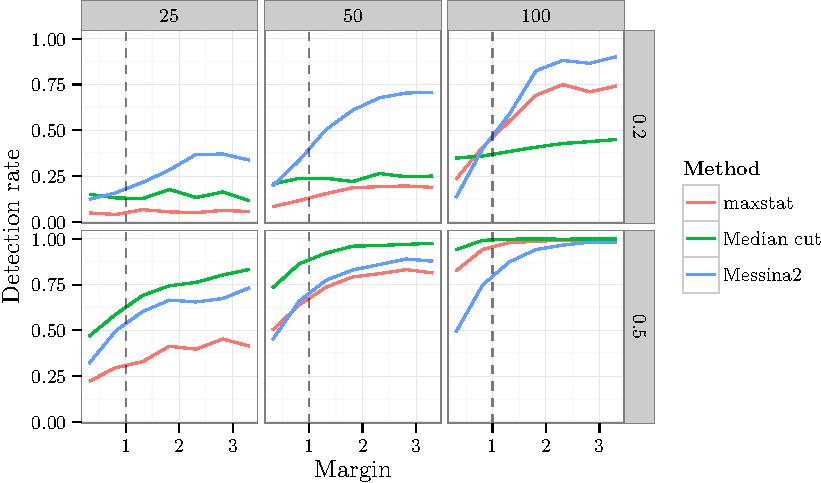
\includegraphics[width=\maxwidth]{figure/06-E2B-E2B-plots-1} 

}


\begin{kframe}\begin{alltt}
\hlkwd{ggplot}\hlstd{(e2b.design[e2b.design}\hlopt{$}\hlstd{n} \hlopt{==} \hlnum{50}\hlstd{,],} \hlkwd{aes}\hlstd{(}\hlkwc{x} \hlstd{= margin,} \hlkwc{y} \hlstd{= detrate,} \hlkwc{colour} \hlstd{=} \hlkwd{factor}\hlstd{(method)))} \hlopt{+} \hlkwd{geom_line}\hlstd{(}\hlkwc{lwd} \hlstd{=} \hlnum{1}\hlstd{)} \hlopt{+} \hlkwd{xlab}\hlstd{(}\hlstr{"Margin"}\hlstd{)} \hlopt{+} \hlkwd{ylab}\hlstd{(}\hlstr{"Detection rate"}\hlstd{)} \hlopt{+} \hlkwd{labs}\hlstd{(}\hlkwc{colour} \hlstd{=} \hlstr{"Method"}\hlstd{)} \hlopt{+} \hlkwd{theme_bw}\hlstd{()} \hlopt{+} \hlkwd{facet_grid}\hlstd{(p1} \hlopt{~} \hlstd{pc} \hlopt{~} \hlstd{R1)}
\end{alltt}
\end{kframe}

{\centering 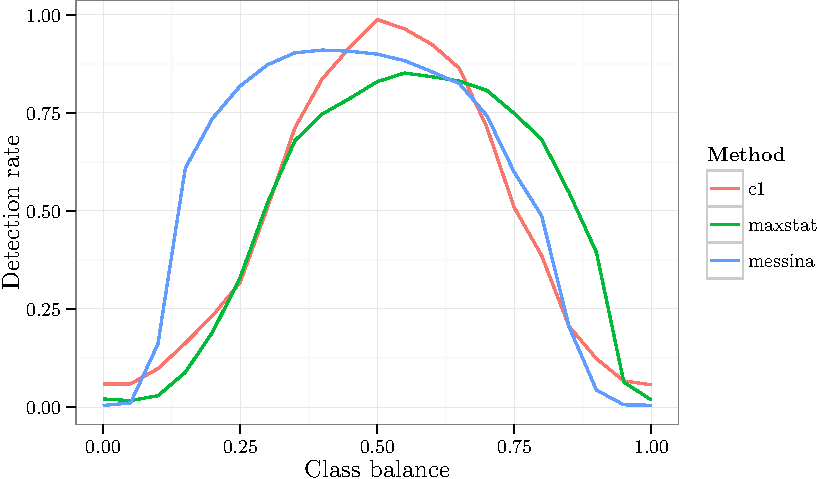
\includegraphics[width=\maxwidth]{figure/06-E2B-E2B-plots-2} 

}


\begin{kframe}\begin{alltt}
\hlkwd{ggplot}\hlstd{(e2b.design[e2b.design}\hlopt{$}\hlstd{n} \hlopt{==} \hlnum{100}\hlstd{,],} \hlkwd{aes}\hlstd{(}\hlkwc{x} \hlstd{= margin,} \hlkwc{y} \hlstd{= detrate,} \hlkwc{colour} \hlstd{=} \hlkwd{factor}\hlstd{(method)))} \hlopt{+} \hlkwd{geom_line}\hlstd{(}\hlkwc{lwd} \hlstd{=} \hlnum{1}\hlstd{)} \hlopt{+} \hlkwd{xlab}\hlstd{(}\hlstr{"Margin"}\hlstd{)} \hlopt{+} \hlkwd{ylab}\hlstd{(}\hlstr{"Detection rate"}\hlstd{)} \hlopt{+} \hlkwd{labs}\hlstd{(}\hlkwc{colour} \hlstd{=} \hlstr{"Method"}\hlstd{)} \hlopt{+} \hlkwd{theme_bw}\hlstd{()} \hlopt{+} \hlkwd{facet_grid}\hlstd{(p1} \hlopt{~} \hlstd{pc} \hlopt{~} \hlstd{R1)}
\end{alltt}
\end{kframe}

{\centering 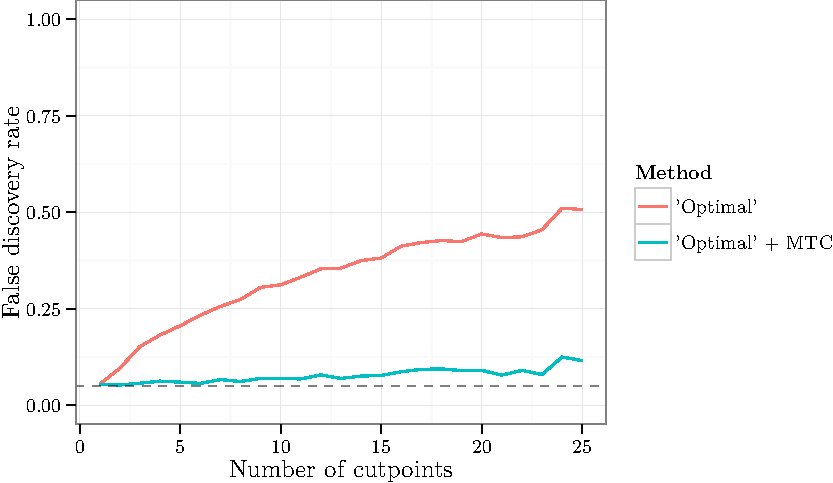
\includegraphics[width=\maxwidth]{figure/06-E2B-E2B-plots-3} 

}


\begin{kframe}\begin{alltt}
\hlkwd{ggplot}\hlstd{(e2b.design2[e2b.design2}\hlopt{$}\hlstd{n} \hlopt{==} \hlnum{25}\hlstd{,],} \hlkwd{aes}\hlstd{(}\hlkwc{x} \hlstd{= margin,} \hlkwc{y} \hlstd{= detrate,} \hlkwc{colour} \hlstd{=} \hlkwd{factor}\hlstd{(method)))} \hlopt{+} \hlkwd{geom_line}\hlstd{(}\hlkwc{lwd} \hlstd{=} \hlnum{1}\hlstd{)} \hlopt{+} \hlkwd{xlab}\hlstd{(}\hlstr{"Margin"}\hlstd{)} \hlopt{+} \hlkwd{ylab}\hlstd{(}\hlstr{"Detection rate"}\hlstd{)} \hlopt{+} \hlkwd{labs}\hlstd{(}\hlkwc{colour} \hlstd{=} \hlstr{"Method"}\hlstd{)} \hlopt{+} \hlkwd{theme_bw}\hlstd{()} \hlopt{+} \hlkwd{facet_grid}\hlstd{(p1} \hlopt{~} \hlstd{pc} \hlopt{~} \hlstd{R1)}
\end{alltt}
\end{kframe}

{\centering 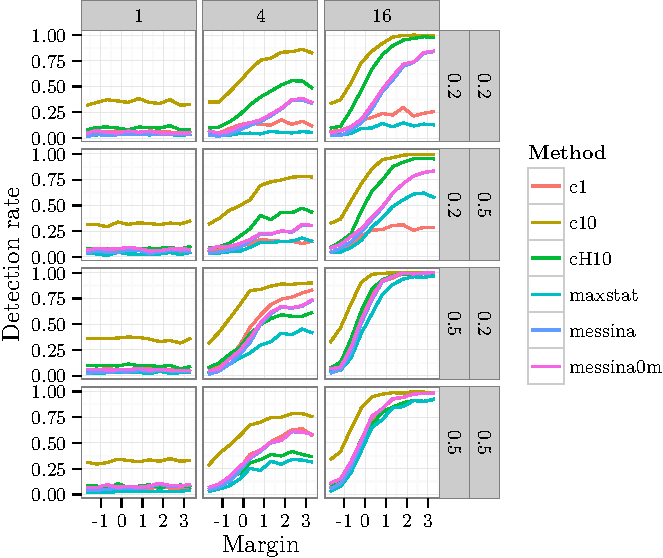
\includegraphics[width=\maxwidth]{figure/06-E2B-E2B-plots-4} 

}


\begin{kframe}\begin{alltt}
\hlkwd{ggplot}\hlstd{(e2b.design2[e2b.design2}\hlopt{$}\hlstd{n} \hlopt{==} \hlnum{50}\hlstd{,],} \hlkwd{aes}\hlstd{(}\hlkwc{x} \hlstd{= margin,} \hlkwc{y} \hlstd{= detrate,} \hlkwc{colour} \hlstd{=} \hlkwd{factor}\hlstd{(method)))} \hlopt{+} \hlkwd{geom_line}\hlstd{(}\hlkwc{lwd} \hlstd{=} \hlnum{1}\hlstd{)} \hlopt{+} \hlkwd{xlab}\hlstd{(}\hlstr{"Margin"}\hlstd{)} \hlopt{+} \hlkwd{ylab}\hlstd{(}\hlstr{"Detection rate"}\hlstd{)} \hlopt{+} \hlkwd{labs}\hlstd{(}\hlkwc{colour} \hlstd{=} \hlstr{"Method"}\hlstd{)} \hlopt{+} \hlkwd{theme_bw}\hlstd{()} \hlopt{+} \hlkwd{facet_grid}\hlstd{(p1} \hlopt{~} \hlstd{pc} \hlopt{~} \hlstd{R1)}
\end{alltt}
\end{kframe}

{\centering 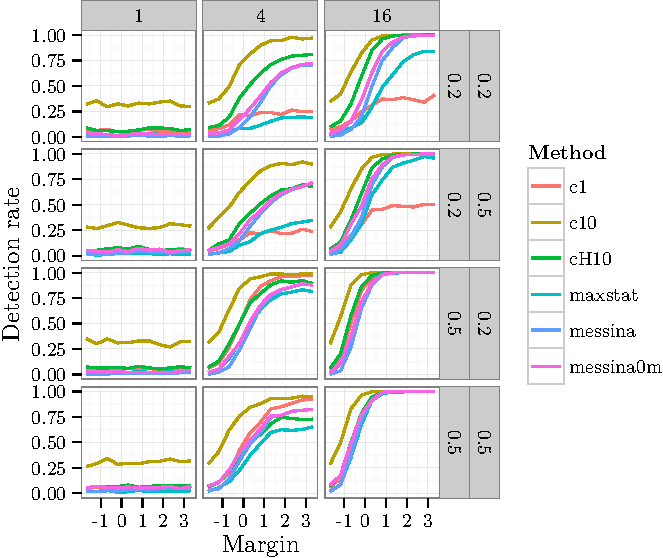
\includegraphics[width=\maxwidth]{figure/06-E2B-E2B-plots-5} 

}


\begin{kframe}\begin{alltt}
\hlkwd{ggplot}\hlstd{(e2b.design2[e2b.design2}\hlopt{$}\hlstd{n} \hlopt{==} \hlnum{100}\hlstd{,],} \hlkwd{aes}\hlstd{(}\hlkwc{x} \hlstd{= margin,} \hlkwc{y} \hlstd{= detrate,} \hlkwc{colour} \hlstd{=} \hlkwd{factor}\hlstd{(method)))} \hlopt{+} \hlkwd{geom_line}\hlstd{(}\hlkwc{lwd} \hlstd{=} \hlnum{1}\hlstd{)} \hlopt{+} \hlkwd{xlab}\hlstd{(}\hlstr{"Margin"}\hlstd{)} \hlopt{+} \hlkwd{ylab}\hlstd{(}\hlstr{"Detection rate"}\hlstd{)} \hlopt{+} \hlkwd{labs}\hlstd{(}\hlkwc{colour} \hlstd{=} \hlstr{"Method"}\hlstd{)} \hlopt{+} \hlkwd{theme_bw}\hlstd{()} \hlopt{+} \hlkwd{facet_grid}\hlstd{(p1} \hlopt{~} \hlstd{pc} \hlopt{~} \hlstd{R1)}
\end{alltt}
\end{kframe}

{\centering 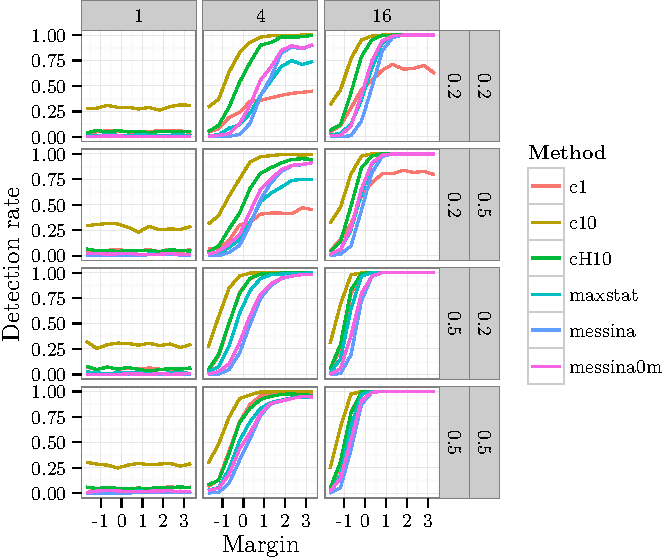
\includegraphics[width=\maxwidth]{figure/06-E2B-E2B-plots-6} 

}


\begin{kframe}\begin{alltt}
\hlkwd{ggplot}\hlstd{(e2b.design3[e2b.design3}\hlopt{$}\hlstd{method} \hlopt \hlkwd{c}\hlstd{(}\hlstr{"c1"}\hlstd{,} \hlstr{"maxstat"}\hlstd{,} \hlstr{"messina"}\hlstd{),],} \hlkwd{aes}\hlstd{(}\hlkwc{x} \hlstd{= p1,} \hlkwc{y} \hlstd{= detrate,} \hlkwc{colour} \hlstd{=} \hlkwd{factor}\hlstd{(method)))} \hlopt{+} \hlkwd{geom_line}\hlstd{(}\hlkwc{lwd} \hlstd{=} \hlnum{1}\hlstd{)} \hlopt{+} \hlkwd{xlab}\hlstd{(}\hlstr{"Class balance"}\hlstd{)} \hlopt{+} \hlkwd{ylab}\hlstd{(}\hlstr{"Detection rate"}\hlstd{)} \hlopt{+} \hlkwd{labs}\hlstd{(}\hlkwc{colour} \hlstd{=} \hlstr{"Method"}\hlstd{)} \hlopt{+} \hlkwd{theme_bw}\hlstd{()}
\end{alltt}
\end{kframe}

{\centering 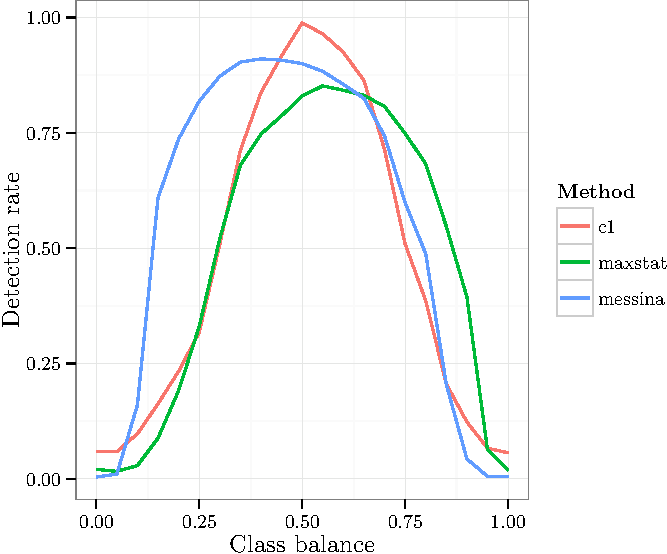
\includegraphics[width=\maxwidth]{figure/06-E2B-E2B-plots-7} 

}


\begin{kframe}\begin{alltt}
\hlkwd{ggplot}\hlstd{(e2b.design4,} \hlkwd{aes}\hlstd{(}\hlkwc{x} \hlstd{= multicut.n,} \hlkwc{y} \hlstd{= detrate,} \hlkwc{colour} \hlstd{=} \hlkwd{factor}\hlstd{(method)))} \hlopt{+} \hlkwd{geom_line}\hlstd{(}\hlkwc{lwd} \hlstd{=} \hlnum{1}\hlstd{)} \hlopt{+} \hlkwd{xlab}\hlstd{(}\hlstr{"Number of cutpoints"}\hlstd{)} \hlopt{+} \hlkwd{ylab}\hlstd{(}\hlstr{"False discovery rate"}\hlstd{)} \hlopt{+} \hlkwd{labs}\hlstd{(}\hlkwc{colour} \hlstd{=} \hlstr{"Method"}\hlstd{)} \hlopt{+} \hlkwd{theme_bw}\hlstd{()} \hlopt{+} \hlkwd{ylim}\hlstd{(}\hlnum{0}\hlstd{,} \hlnum{1}\hlstd{)} \hlopt{+} \hlkwd{geom_hline}\hlstd{(}\hlkwc{yintercept} \hlstd{=} \hlnum{0.05}\hlstd{,} \hlkwc{linetype} \hlstd{=} \hlstr{"dashed"}\hlstd{,} \hlkwc{alpha} \hlstd{=} \hlnum{0.5}\hlstd{)}
\end{alltt}
\end{kframe}

{\centering 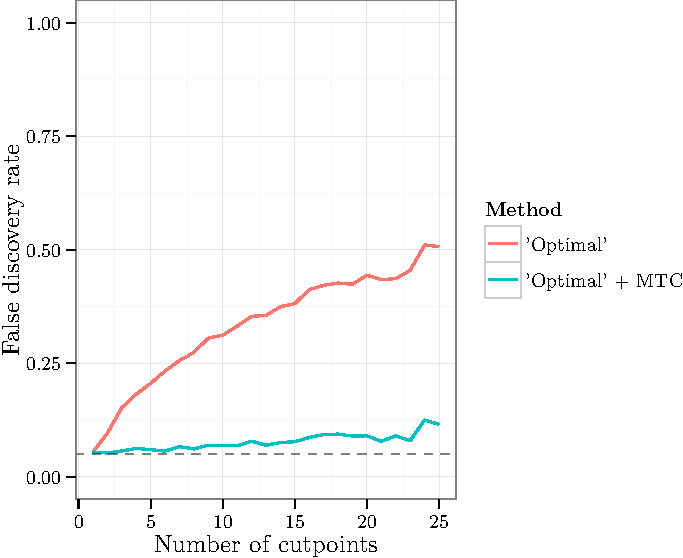
\includegraphics[width=\maxwidth]{figure/06-E2B-E2B-plots-8} 

}



\end{knitrout}

\end{document}
